%%%%%%%%%%%%%%%%%%%%%%%%%%%%%%%%%%%%%%%%%%%%%%%%%%%%%%%%%%%%%%%%%%
%        Contents: Bachelorarbeit, HS Fulda        %
%                          06.09.2022                        %
%---------------------------------------------------------%
%                     Implementierung.tex               %
%                        by Fangfang Tan                    %
%         fangfang.tan@informatik.hs-fulda.de      %
%%%%%%%%%%%%%%%%%%%%%%%%%%%%%%%%%%%%%%%%%%%%%%%%%%%%%%%%%%%%%%%%%%

\chapter{Implementierung des Anwendungsfalls} \label{IM}


In Abschnitt 1.3 wurden die Anforderungen an die zu implementierende Anwendung bereits vorgestellt, in diesem Kapitel wird nun die Umsetzung in den einzelnen Technologien (Fiori Elements in Kombination mit SAP CAP, AppGyver und SAPUI5) näher beschrieben. 

\begin{table}[htbp]
  \centering
	\begin{tabular}{|l|l|l|} 
	\hline 
	\rowcolor{gray!40}
     Technologie&Frontend&Backend\\
	\hline  
	AppGyver&X&-\\
	\hline
	SAPUI5&X&-\\
	\hline
	Fiori Elements (inkl. SAP CAP)&X&X\\
	\hline
	\end{tabular}
  \caption{Umsetzungsanforderung der Technologien} 
\end{table}

Dabei ist zwischen Backend- und Frontend-Funktionalität zu unterscheiden. SAPUI5 verfügt grundsätzlich über keine Backend-Funktionalität. Mit SAP AppGyver können lokale Datenstrukturen erzeugt werden. Diese Funktion wird jedoch nicht genutzt, stattdessen wird ein zentraler OData-Service inklusive Datenbackend an anderer Stelle bereitgestellt. Hierfür wird auf die „Full Stack“-Anwendungen, bestehend aus Fiori Elements und SAP CAP, im SAP Application Studio zurückgegriffen. Das Fiori Elements-Frontend wird den erstellten OData-Service dann konsumieren. SAP Appgyver und SAPUI5 nutzen hier das gleiche Datenmodell und den gleichen OData-Service. 

\begin{figure}[htbp]
 \centering
 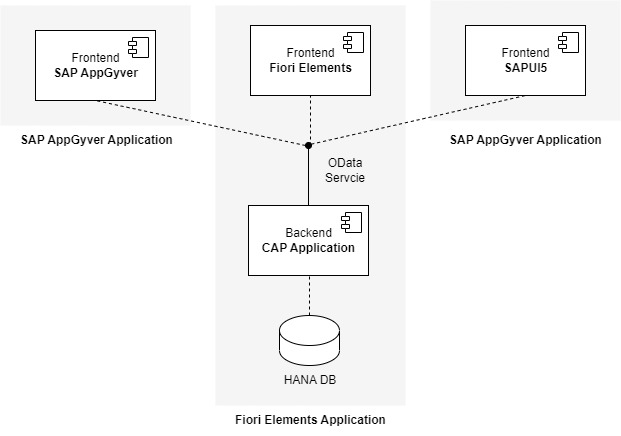
\includegraphics[width=0.7\textwidth]{Bilder/architecture/apps_architektur.jpg}
 \caption{Umsetzungsarchitektur der Technologien}
\end{figure}

\section{Fiori Elements}
\subsection{Dev Space erstellen}

Für die Entwicklung mit Fiori Elements wird das Business Application Studio als Entwicklungsumgebung genutzt. Wie bereits in Abschnitt 2.6.2 erwähnt, stellt das BAS Dev Spaces für unterschiedliche Entwicklungsszenarien bereit. Die komplette Anwendung ließe sich auch als klassisches Entwicklungsprojekt auf- und umsetzen, im Sinne der Arbeit wird jedoch das “Low-Code-Based Full-Stack Cloud-Application” Preset für den Dev Space gewählt, um Zugriff auf die LCNC-Funktionalitäten zu bekommen. 

\begin{figure}[htbp]
 \centering
 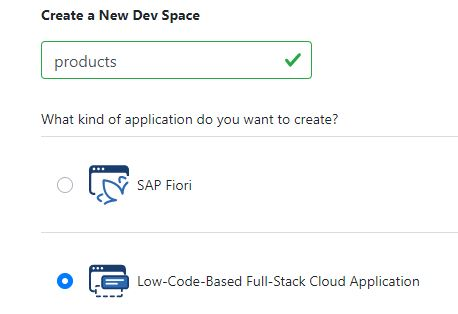
\includegraphics[width=0.6\textwidth]{Bilder/fiori_element/3_2_create dev space.JPG}
 \caption{Create a New Dev Space}
\end{figure}

Nach der Erstellung des Dev Space wird die Entwicklungsumgebung für eine Low-Code-basierte Full-Stack Cloud-Anwendung bereitgestellt. In dieser Umgebung stehen verschiedene „Cards“ zur Verfügung, um den auf Low-Code basierenden Implementierungsprozess durchzuführen.

\begin{figure}[htbp]
 \centering
 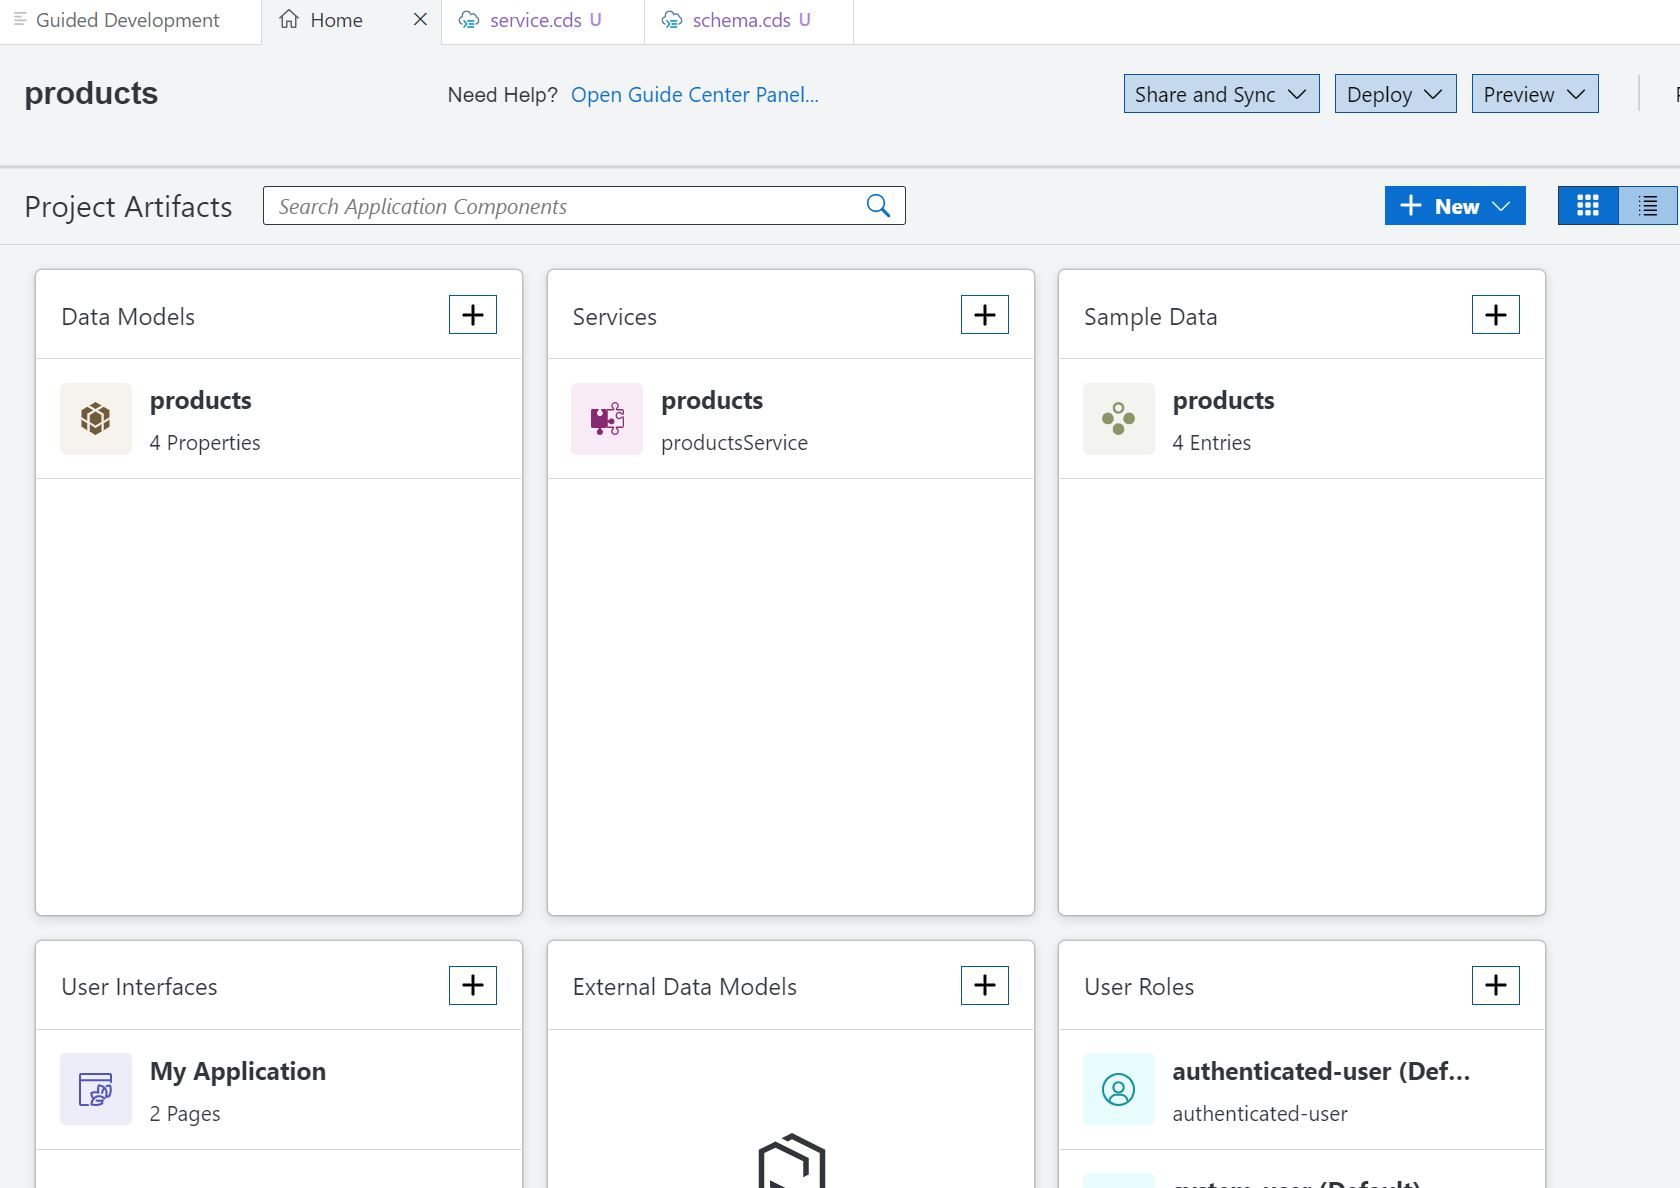
\includegraphics[width=0.8\textwidth]{Bilder/fiori_element/3_3_Cards_von_BAS.JPG}
 \caption{Grundlegenden Aufbau inkl. der Cards von BAS}
\end{figure}

\subsection{Datenentitäten und Service definieren}
Für den Anwendungsfall wird eine Datenentität mit sechs Properties festgelegt. Neue Entitäten können einfach in der Datenmodellkarte hinzugefügt und konfiguriert werden. Der Entitätsname wird als „Products“ definiert und die sechs Properties sind ID, Title, MaterialNumber, Description, Price und Stock. Um die Implementierung des Anwendungsfalls zu erleichtern, wird die ID hier als UUID und alle anderen Properties als String definiert.

\begin{figure}[htbp]
 \centering
 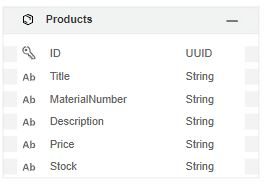
\includegraphics[width=0.5\textwidth]{Bilder/fiori_element/3_4_Data_Model.JPG}
 \caption{Datenmodell}
\end{figure}

Beim Anlegen der Entität über die UI wird im Hintergrund eine Code-Datei erzeugt (model.cds) und die Definition dort abgelegt. Dies ist im LCNC-Modus für den Entwickler nicht sichtbar und er muss sich um das Coding nicht weiter kümmern. Grundsätzlich ist es aber möglich, das Coding manuell anzupassen und die UI reagiert entsprechend auf die Änderungen im Coding. Es ist jedoch herauszustellen, dass die Wizards und UI-Masken von BAS nicht alle Funktionalitäten von SAP CAP unterstützen und so spezielle Dinge ggf. nur über das Coding hinzugefügt werden können. Für den gewählten Use-Case ist dies jedoch nicht von Belang.

Angelegte Datenbank-Entitäten können im Weiteren einfach als OData-Service exponiert werden. Ähnlich wie beim Datenmodell, gibt es dafür eine eigene Karte. Dort wird lediglich die Entität ausgewählt, Name, Namespace und Typ festgelegt, sowie einige weitere Properties konfiguriert und dann kann der Service erstellt werden.

\begin{figure}[htbp]
 \centering
 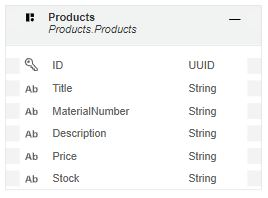
\includegraphics[width=0.5\textwidth]{Bilder/fiori_element/3_5_Service.JPG}
 \caption{Service}
\end{figure}

Unter der Sample-Data-Karte können Mock-Daten hinterlegt werden, damit man während der Entwicklung direkt Zugriff auf Daten hat. Da die Property-ID als UUID definiert ist, werden die IDs automatisch vom System vergeben. Die anderen Properties wie Title, MaterialNumber, Description, Price und Stock müssen manuell eingetragen werden.

\begin{figure}[htbp]
 \centering
 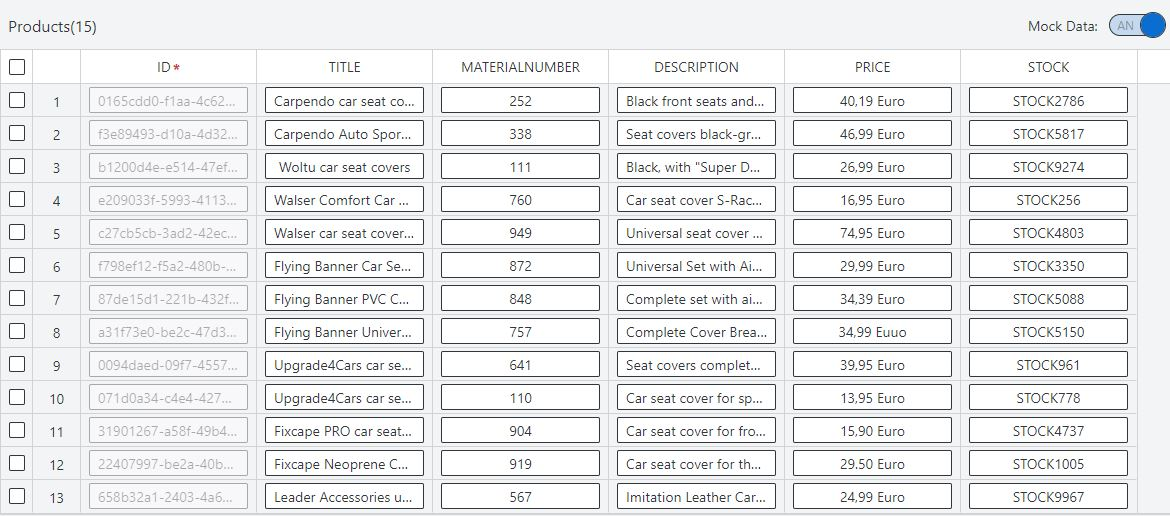
\includegraphics[width=1.0\textwidth]{Bilder/fiori_element/3_6_Sample_Data.JPG}
 \caption{Sample Data}
\end{figure}

Tatsächlich hat man durch die Verwendung der drei Cards mit diesen wenigen Klicks und Eingaben in sehr kurzer Zeit ein eigenes Datenmodell und einen OData-Service definiert, den man in der Preview im BAS auch direkt aufrufen und testen kann.

\subsection{User Interface erstellen }

Die Anforderungen an die Benutzeroberfläche bestehen darin, dass eine Listenansicht für die Anzeige aller Produkte und eine Einzelansicht für ein einzelnes Produkt, sowie eine Maske für die Pflege jedes einzelnen Produkts entworfen werden sollen. SAP Fiori Elements stellt hierfür bereits komplett vorgefertigte Floorplans zur Verfügung, die nahtlos in BAS integriert sind.
Unter der User-Interfaces-Karte kann die Benutzeroberfläche der Anwendung definiert werden. Dies erfolgt in vier Schritten: 

\begin{enumerate}
\item Eingabe der Details der UI-Anwendung wie Name und Namespace.
\item Auswahl des Anwendungstyps. In dem hier vorgestellten Anwendungsfall wird eine \textit{Template-Based, Responsive Application} ausgesucht. Es wäre jedoch auch möglich, eine Freestyle SAPUI5-Anwendung zu erstellen.
\item Wie in Abschnitt 2.6.1 erwähnt, werden von SAP verschiedene Arten von Floorplans für Fiori Elements bereitgestellt. In diesem Fall wird \textit{List Report Object Page} für UI Application Template verwendet.
\item Der letzte Schritt bei der Erstellung einer UI-Anwendung ist die Auswahl des richtigen Datenobjekts. Hier wird die Datenentität \textit{Products} gewählt und es werden automatisch Tabellenspalten zur Listenseite und ein Abschnitt zur Objektseite eingeschaltet. 
\end{enumerate}

\begin{figure}[htbp]
 \centering
 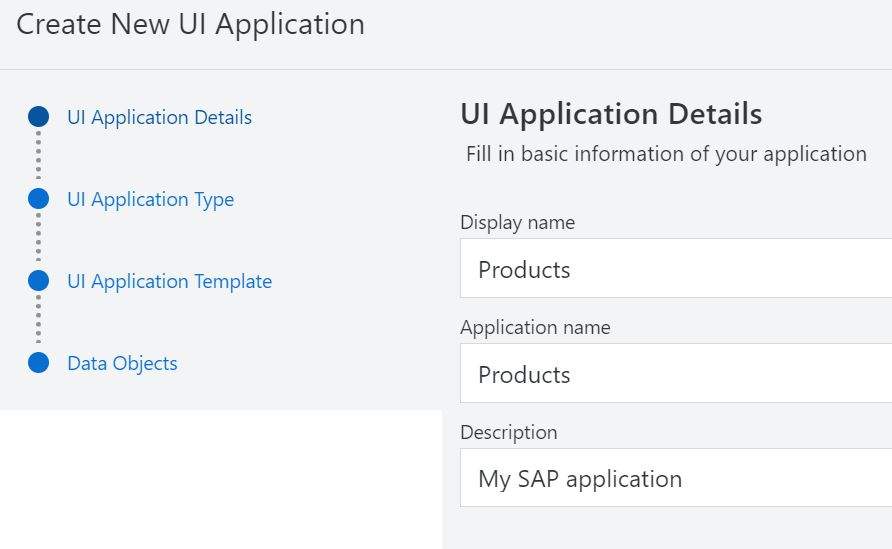
\includegraphics[width=0.7\textwidth]{Bilder/fiori_element/3_7_UI_Konfiguration.jpg}
 \caption{UI-Konfiguration}
\end{figure}

Nach dem Klick auf den „Finish“-Button wird die UI-Application automatisch generiert. Auch hier wird im Hintergrund Quellcode abgelegt: Zum einen werden die OData-Annotationen in weiteren cds-Dateien abgelegt. Das Weiteren wird das Grundgerüst einer SAPUI5-Anwendung angelegt und mit der entsprechenden Konfiguration für SAP Fiori Elements versehen. Auch dies ist für den Entwickler nicht direkt in BAS einsehbar, bzw. es ist nicht notwendig sich mit dem Code auseinander zu setzen, es sei denn, man möchte gezielt Funktionen nutzen, die von den Wizards in BAS nicht unterstützt werden.
Die finale Anwendung besteht aus einer Listenseite und einer Detailseite für jedes Produkt. Die Listenseite zeigt eine Liste aller Produkte. Wird auf ein Listenelement geklickt, so wird die Detailseite für das jeweilige Produkt geöffnet. Zudem kann ein neues Produkt hinzugefügt, ein Produkt gelöscht oder bearbeitet werden.  Während man über die Konfiguration einen Einfluss auf die Tabellenspalten und Inhalte der Einzelansicht nehmen kann, funktionieren Dinge wie Navigation, Daten laden, Datenbindung und auch das Speichern von neuen Datensätzen einfach so, ohne, dass vom Entwickler irgendeine komplexere Konfiguration vorgenommen werden muss. Allerdings kann man von dem Standardverhalten auch nicht abweichen und jede Anwendung folgt dem grundlegenden Aufbau und Verhalten des ausgewählten Floorplans.
Mithilfe der Page Map in BAS kann die UI-Anwendung angepasst werden. Zum Beispiel können für die hier vorgestellte Anwendung das initiale Laden aktiviert werden und auch die Properties, die in der Liste angezeigt werden, können je nach Anforderung geändert werden. Dabei sind alle Parameter über UI-Masken konfigurierbar und an keiner Stelle muss ein eigenes Coding erfolgen.


\begin{figure}[htbp]
 \centering
 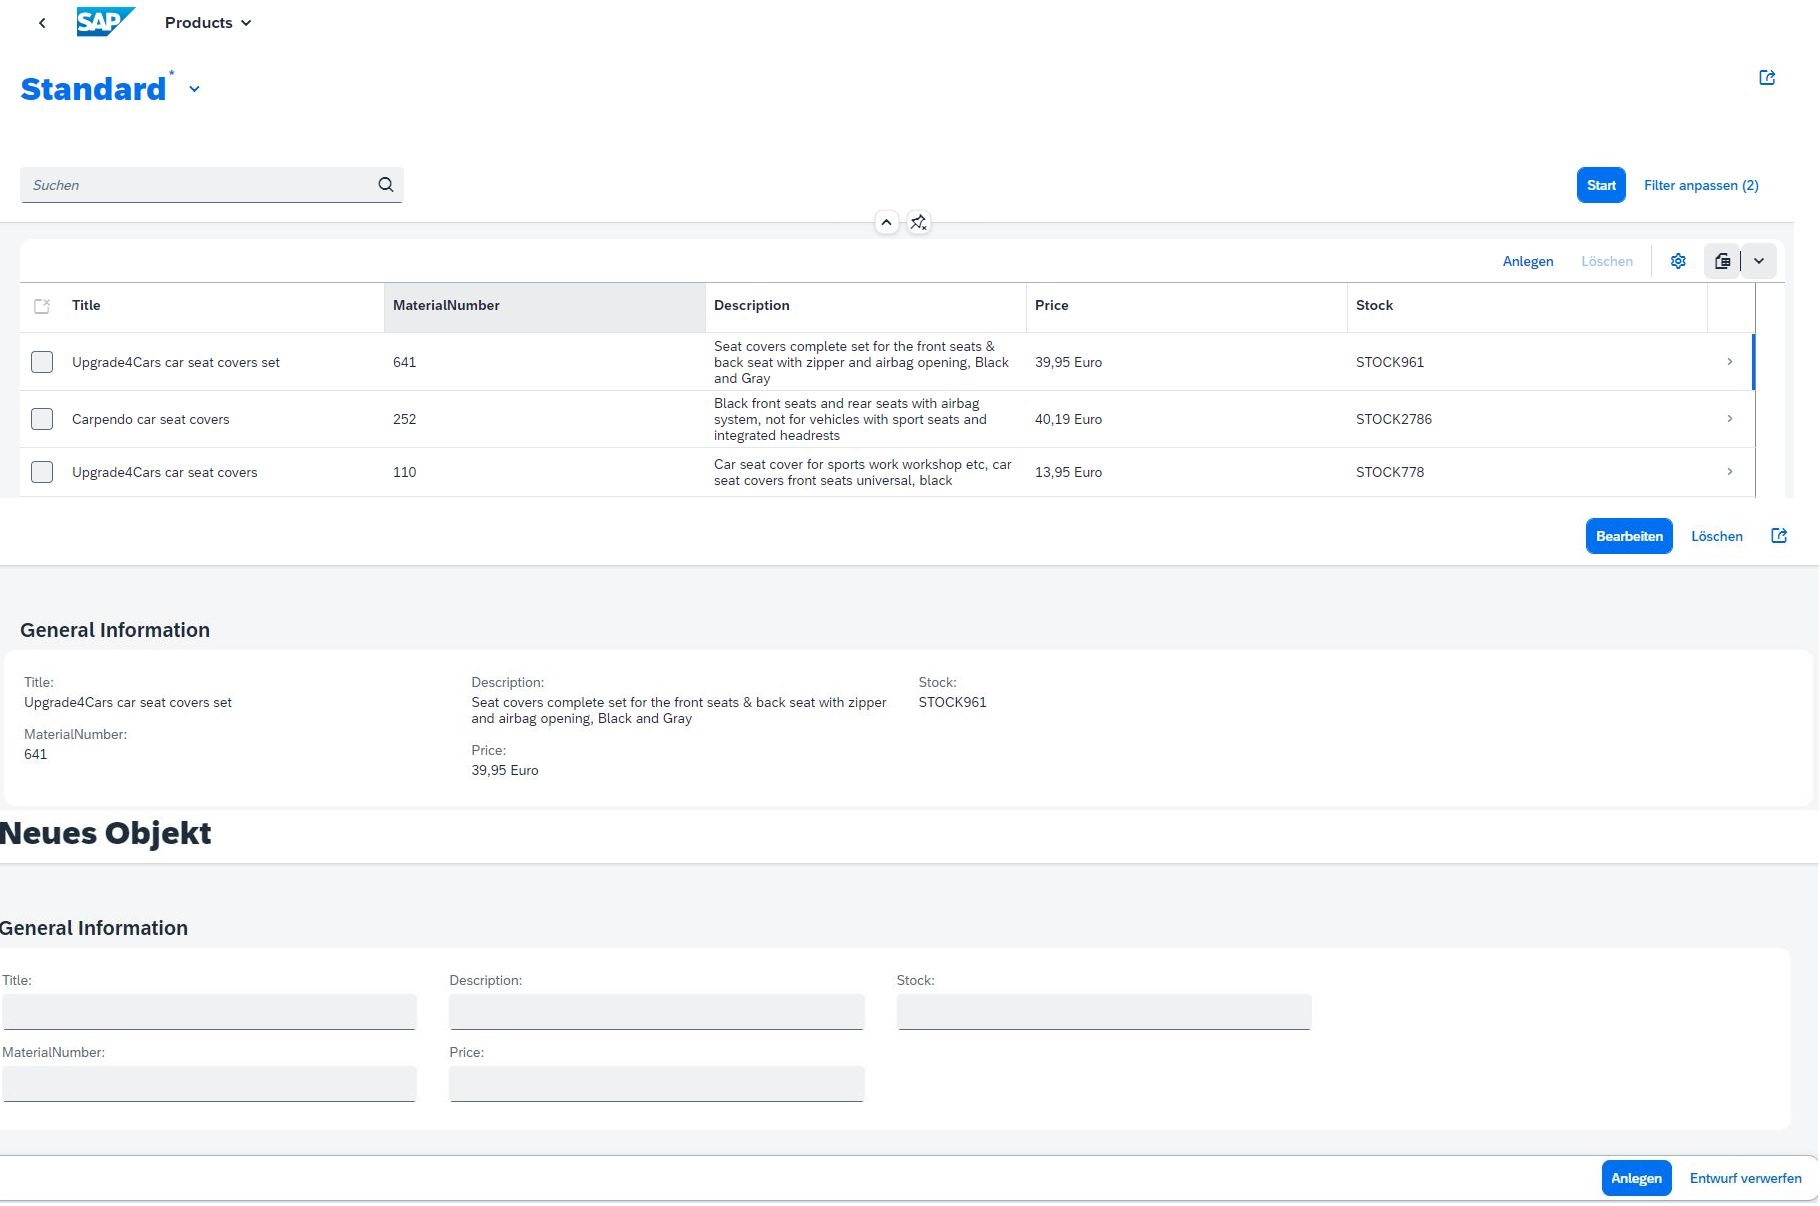
\includegraphics[width=1.0\textwidth]{Bilder/fiori_element/3_8_Fiori_Element_list.jpg}
 \caption{Listenseite, Detailseite und „neues Objekt anlegen Seite der Fiori-Elements-Anwendung}
\end{figure}

\subsection{Deployment des OData-Services}

Um auf den OData-Service auch aus den anderen Applikationen zuzugreifen und die UI-Anwendung bereitzustellen, muss ein Deployment aus BAS heraus erfolgen. Das Deployment erfolgt direkt auf die SAP BTP. Hierfür muss ein sogenannter „Space“ auf der SAP Business Technology Plattform vorliegen, sowie eine SAP HANA Cloud-Instanz bereitgestellt werden. Nachdem die Anwendungsbenutzeroberfläche in Business Application Studio erstellt worden ist, kann diese, ohne der Notwendigkeit von zusätzlichem Coding, direkt aus dem BAS heraus deployed werden. Dazu muss man in BAS bei Cloud Foundry anmelden und das Cloud Foundry-Ziel angeben. Abbildung 3.9 zeigt, wie dies geht. 

\begin{figure}[htbp]
 \centering
 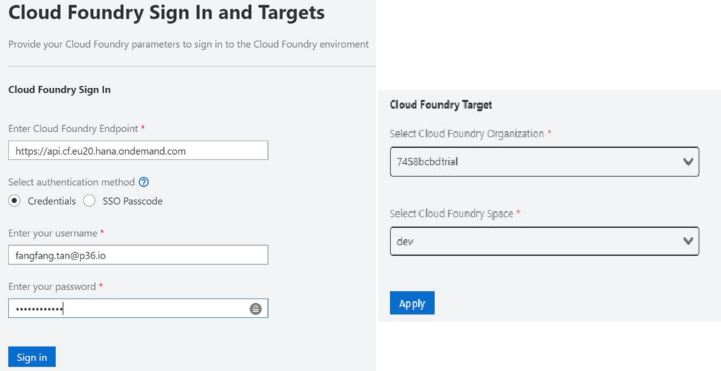
\includegraphics[width=0.9\textwidth]{Bilder/fiori_element/3_9_cloud_foundry_targets.jpg}
 \caption{Cloud Foundry Sign In und Targets}
\end{figure}

Danach lässt sich das Deployment starten und es werden während des Vorgangs alle notwendigen Komponenten (Applikation und notwendige BTP-Servie-Instanzen) erstellt. Nach dem Deployment stehen OData-Service, sowie UI-Applikation dann unter einer URL zur Verfügung.
Auch das Deployment erfolgt vollständig als No-Code-Ansatz. Die notwendige Konfigurationsdatei (mta.yml) wird im Hintergrund des Projekts abgelegt und beim Deployment ausgelesen. Während der Implementierung gab es jedoch gelegentlich Probleme bei dem Deployment, sodass eine tiefergehende Analyse erforderlich wurde. Insbesondere in solchen Fällen musste die LCNC-Umgebung verlassen werden, damit in den Log-Dateien der Fehler gefunden werden konnte. Zudem waren die Probleme meist sehr technischer Natur und erforderten ein tiefgreifenderes Verständnis der verwendeten Technologien (SAP CAP, SAP BTP).

\section{AppGyver}
\subsection{Projektaufbau}

Für die Umsetzung des Projekts wird SAP AppGyver Enterprise auf der SAP BTP verwendet. Die notwendigen Services können einfach in der SAP BTP aktiviert werden und nach Zuweisung der entsprechenden Rollen steht die Composer Pro-Entwicklungsplattform bereit.

\subsection{OData Integration}

Seit dem Kauf durch SAP wird SAP AppGyver immer mehr in das Ökosystem der SAP integriert. So ist es in der Enterprise-Edition mittlerweile möglich, Funktionen der SAP BTP zu nutzen, um Daten in AppGyver bereitzustellen. Um die Daten des OData-Services in AppGyver nutzen zu können, muss eine „Destination“ im SAP Business Technology Plattform Cockpit angelegt werden. Der SAP BTP Connectivity Service stellt via Destinations Reverse Proxy- und Authentifizierungsfunktionen zur Verfügung, sodass unter Verwendung der Destination ein einfacherer Zugriff auf einen Remote-Endpunkt erfolgen kann. Die Verbindungsdetails können via Eingabemaske gepflegt werden \cite{shp:dest}. Anzugeben sind Name, eine URL, Authentifizierungsdetails sowie weitere spezifische Konfigurationsparameter. Die Destination wird hier \textit{products-on-trial\_simple} genannt. Die URL bezieht sich auf die OData-Service-Adresse. Die Authentifizierung wird dann als „OAuth Client Credentials Authentication“ definiert. Wichtig ist, dass die „Additional Properties“ gesetzt werden: \textit{AppgyverEnabled} sowie \textit{HTML5.DynamicDestination} müssen auf \textit{true} gesetzt werden, damit der OData-Service in AppGyver eingebunden werden kann.

\begin{figure}[htbp]
 \centering
 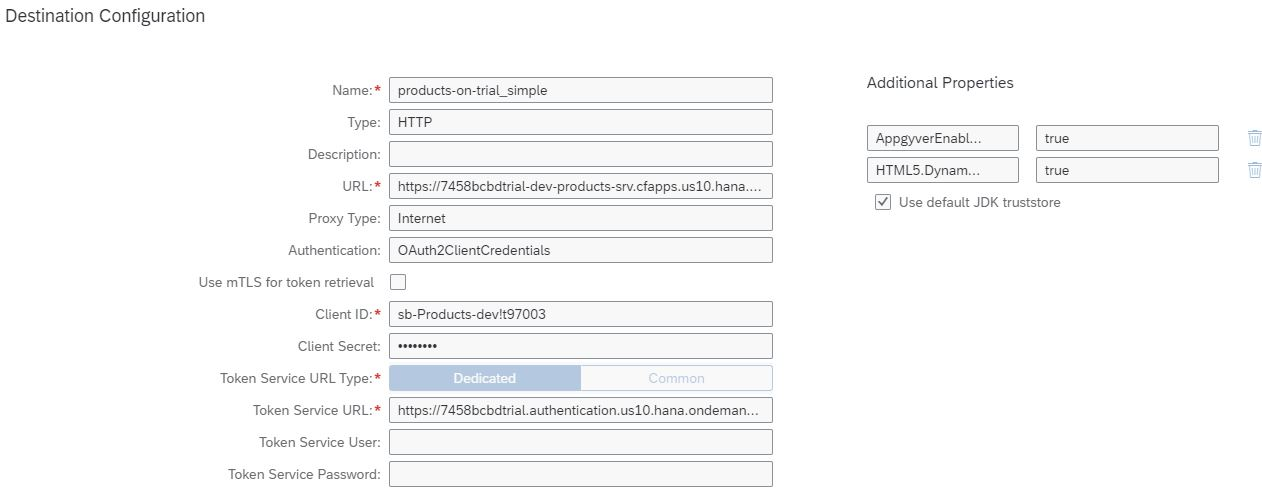
\includegraphics[width=1.0\textwidth]{Bilder/appgyver/3_10_destination.jpg}
 \caption{Destination-Konfiguration in SAP BTP Cockpit}
\end{figure}

Nachdem die Destination erstellt wurde, ist der Service \textit{products-on-trial\_simple} in SAP AppGyver unter dem Menüpunkt Data – SAP Systems verfügbar und kann importiert werden. AppGyver verfügt über eine Funktionalität zum Auslesen der Metadaten des OData-Services und listet die vorhandenen Entitäten in der UI auf. Die Entität „Products“ kann dann einfach aktiviert werden und steht dann in der Anwendung zur Verfügung. Bereits im Integrations-Wizard lassen sich Dateninhalte und Werte des OData-Services ansehen, bzw. sogar verändern.

\begin{figure}[htbp]
 \centering
 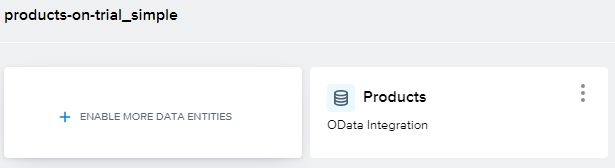
\includegraphics[width=0.7\textwidth]{Bilder/appgyver/3_11_odata integration_in_AppGyver.jpg}
 \caption{OData-Integration in AppGyver}
\end{figure}

\subsection{Listenansicht zur Anzeige aller Produkte}
Um eine Liste aller Produkte anzeigen zu können, muss zunächst eine Listenseite mit dem Namen „The List of Products“ erstellt werden. Diese Seite besteht aus vier Elementen: Einem Titel mit dem Text „Products“, einem Button zum Erstellen eines neuen Produkt-Datensatzes und einem weiteren Button zum Einblenden eines Suchfeldes, sowie einem List Item. Die Erstellung eines Suchfeldes wird in Kapital 4 näher betrachtet werden. Eine Data-Variable mit dem Namen „Product1“ wird erstellt, um die Daten von OData-Service abzurufen. Der Typ der Data-Variablen ist auf „Collection of data records“ eingestellt, wodurch eine Sammlung von Datensätzen geliefert wird. Die Data-Variable verfügt über eine Default-Logik, die bestimmt, wie sie sich mit Daten aus dem Backend füllt. Die Daten werden aus dem Backend über den Ablauffunktionskomponente „Get record collection“ bezogen, wobei die Daten hier nur als ein Ausgangsargument des Knotens existieren. Dann wird den „Set data variable“-Ablauffunktionskomponente verwendet, damit die Daten in die Data-Variable setzen können. Nun steht die Data-Variable \textit{Product1} für die Verwendung in View-Componente Binding zur Verfügung.

\begin{figure}[htbp]
 \centering
 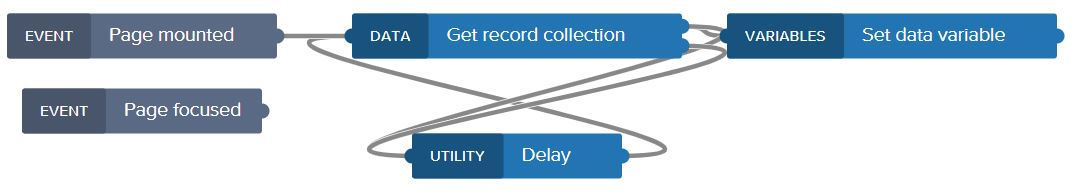
\includegraphics[width=1.0\textwidth]{Bilder/appgyver/3_12_Data_Variable_Logik.jpg}
 \caption{Data-Variable Logik}
\end{figure}

Zur Anzeige der Produkteliste muss die View-Component „List item“ mit dem erstellten Data-Variable \textit{Product1} verbunden und  wiederholt werden. Das Primary  und das Secondary Label bestimmen, welcher Property-Wert in der Liste angezeigt werden soll. In dieser AppGyver-Anwendung sollen der Produkttitel und der Produktpreis angezeigt werden. Deshalb sollten das Primary Label mit dem Wert \textit{current.Title} und das Secondary Label mit \textit{current.Price} verbunden werden. Nach dem Speichern wird dann die Liste mit allen Produkten angezeigt.  

\begin{figure}[htbp]
 \centering
 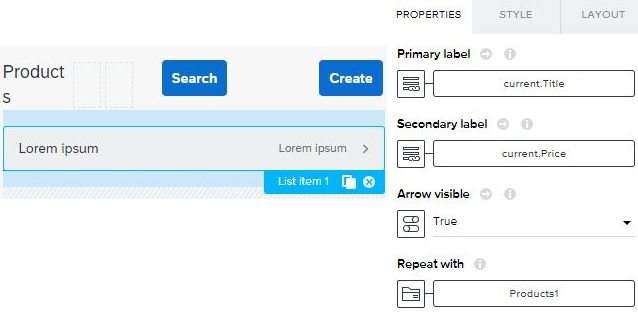
\includegraphics[width=0.7\textwidth]{Bilder/appgyver/3_13_List_Item_mit_Repeat.jpg}
 \caption{Listenseite und List Item mit Repeat in AppGyver}
\end{figure}

\subsection{Einzelansicht für ein Produkt}
Die Einzelansicht enthält alle Properties zu einem Produkt, nämlich den Produkttitel, die Beschreibung, die Materialnummer, den Preis, den Bestand und die Produkt-ID. Für die Darstellung der Informationen muss eine Detailseite mit dem Namen „Product Details“ erstellt werden. Eine App-Variable \textit{appVarRecord} mit sechs Properties wird erstellt, damit die Daten an verschiedene Seiten der Anwendung übertragen werden können.

Um von der Listenseite zur Detail-Seite zu navigieren, muss die logische Ablauffunktion für das List Item in der Listenseite aufgebaut werden. Hierbei geht es um ein Component tap Event. Das Event wird ausgelöst, wenn das List Item vom Benutzer angeklickt wird. Der Aufbau der logischen Ablauffunktion kann Abbildung 3.14 entnommen werden. 
\begin{figure}[htbp]
 \centering
 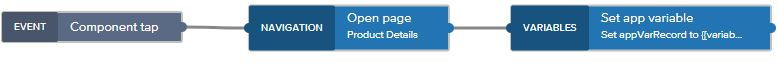
\includegraphics[width=0.9\textwidth]{Bilder/appgyver/3_14_Logik_ListItem.JPG}
 \caption{Logische Ablauffunktion für List Items}
\end{figure}

Eine „Open page“-Ablauffunktionskomponente ist erforderlich, um die Detailseite zu öffnen. Die Ausgangspunkte der Ablauffunktionskomponente „Open page“ sind mit der Ablauffunktionskomponente „Set app variable“ verknüpft. Mit dieser Komponente werden die Daten in dem List Item mit der neu angelegten App-Variable verbunden. Die Werte der Properties von der App-Variable werden mit den jeweiligen Property-Werten in Wiederholung von List Item gesetzt. Dabei handelt es sich um die Werte der Data-Variablen \textit{Products1}. Da die Werte der Date-Variablen \textit{Product1} mit dem OData Service verbunden wurden, wird der Wert aus dem Backend in die App-Variable eingesetzt.

\begin{figure}[htbp]
 \centering
 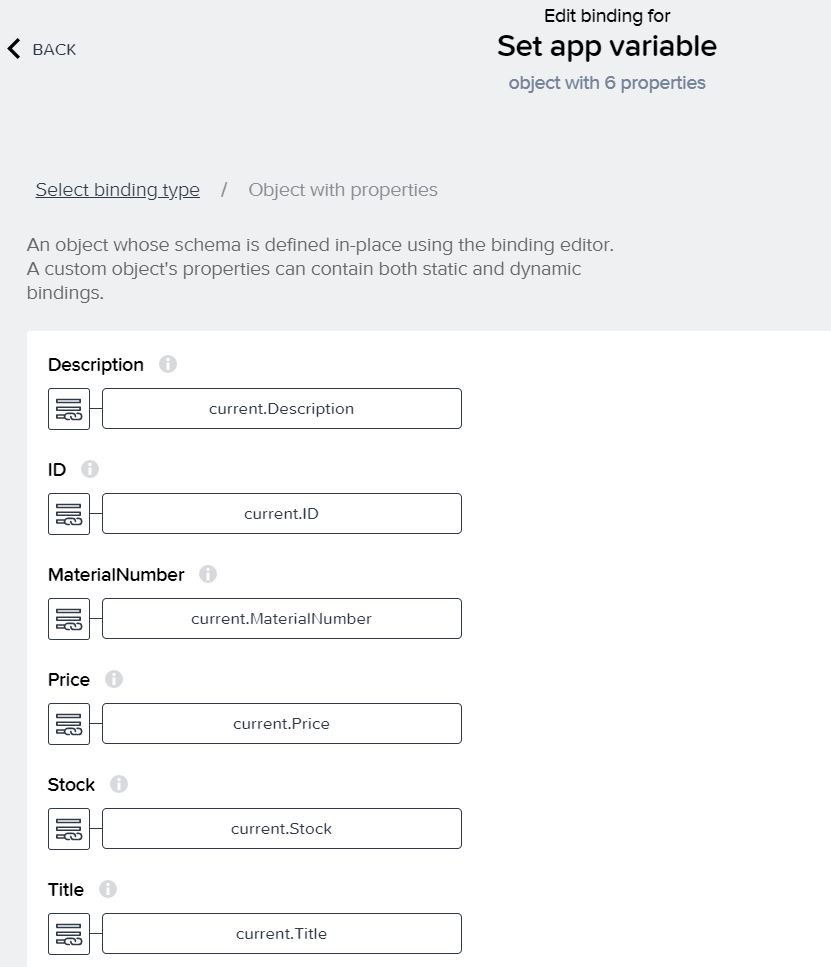
\includegraphics[width=0.5\textwidth]{Bilder/appgyver/3_15_set_app_variable.JPG}
 \caption{Wert zuweisen für App-Variable \textit{appVarRecord} in \textit{Set app variable} Ablauffunktionskomponente}
\end{figure}

Auf der Detailseite werden sechs Input-Felder erstellt. Die Werte der Input-Felder sind mit dem entsprechenden Property-Wert der App-Variablen \textit{appVarRecord} verbunden, nämlich dem Titel, der Materialnummer, dem Preis, der Produkt-ID und der Beschreibung sowie dem Bestand. Außerdem werden drei Buttons für 3 Component tap Events auf der Detailseite erstellt: Der „Back“-Button wird verwendet, um zurück zur Listenseite zu navigieren. Um dies zu implementieren, muss lediglich eine Logikablauffunktion mit der Komponente „Navigation back“ erstellt werden (vgl. Abb. 3.16). Der „Edit“-Button wird zum Aktualisieren der Produktinformationen genutzt. Dazu ist die in Abbildung 3.16 dargestellte Ablauffunktion mit der Komponente „Update record“ erforderlich. Die Ablauffunktionskomponente ist mit der Datenressource Products (vgl. Abb. 3.11) und der App-Variablen \textit{appVarRecord} verknüpft. Die „Update record“-Komponente hat zwei Ausgänge: Der obere ist mit einer „Alert“-Ablauffunktionskomponente verlinkt, die zur Anzeige von „Update Record ID“ dient, der untere ist mit einer „Toast“-Ablauffunktion verbunden, die nur benutzt wird, wenn die Aktualisierung des Datensatzes nicht erfolgreich abgeschlossen werden kann. Der „Delete“-Button in Kombination mit der „Delete record“-Komponente wird zum Löschen eines Produkts eingesetzt.

\begin{figure}[htbp]
 \centering
 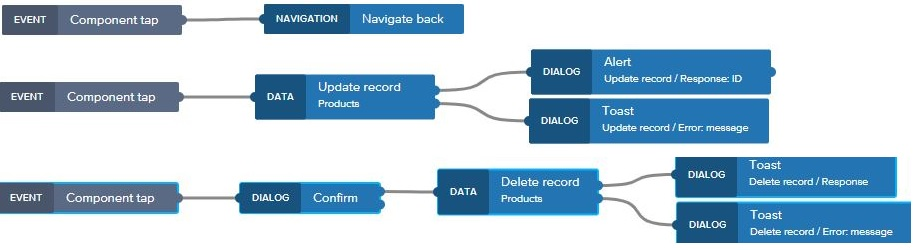
\includegraphics[width=0.9\textwidth]{Bilder/appgyver/3_16_button_logic.jpg}
 \caption{Logische Ablauffunktion für Edit-, Back- und Delete-Button}
\end{figure}

\subsection{Maske zum Erstellen eines einzelnen Produkts}
Zunächst muss eine Seite mit dem Namen „Create New Record“ erstellt werden. Diese Seite besteht aus fünf Input-Feldern, einem „Save“-Button sowie einem „Back“-Button. Eine neue Data-Variable mit dem Variablentyp „New data record“ wird erstellt, die ebenfalls mit der Data-Ressource Products verbunden wird. Data-Variable mit dem Typ „New data record“ initialisiert eine leere Data-Variable, die beim Erstellen eines Formulars zum Anlegen von Datensätzen im Backend zu verwenden ist. Die Werte der Input-Felder werden mit den entsprechenden Property-Werten der Data-Variablen verknüpft. Da die Produkt-ID als UUID definiert ist und vom System generiert wird, muss das Input-Feld dafür nicht erstellt werden.

Um den Datensatz speichern zu können, wird eine Ablauffunktion mit der Komponente „Create record“ für den „Save“-Button benötigt. Ähnlich wie die Ablauffunktionskomponente „Update record“ ist die Komponente „Create record“ mit der Datenressource Products und der App-Variablen appVarRecord verbunden. Sie hat ebenfalls zwei Ausgänge: einen für die Bestätigung der erfolgreichen Erstellung von Datensätzen und einen anderen für die Anzeige des Fehlers (vgl. Abb. 3.17). Der „Back“-Button kann für die Navigation zurück zur Listenseite genutzt werden.

\begin{figure}[htbp]
 \centering
 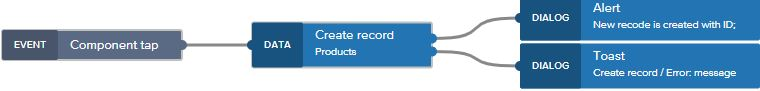
\includegraphics[width=0.9\textwidth]{Bilder/appgyver/3_17_logik_Save_Button.jpg}
 \caption{Logische Ablauffunktion für Save-Button}
\end{figure}

Wie bereits in Kapitel 2.4.2 vorgestellt, lassen sich die AppGyver-Baustein in 3 Schichten des MVC-Modells unterteilen, nämlich in View-, Controller- und Model-Schichten. Auf der View-Schicht wurden für den Anwendungsfall insgesamt 3 Seiten- und 21 View-Komponenten erstellt, darunter 3 Seitentitel, ein List Item, 11 Input-Felder sowie 7 Buttons. Damit die Buttons und das List Item dynamisch funktionieren, wurden in der Controller-Schicht 8 logische Ablauffunktionen mit Componente tap Event erstellt. In der Model-Schicht wurden 2 Daten-Variablen und eine App-Variable erstellt, um die Daten vom Odata-Service zu holen, die Daten zu aktualisieren und sie an verschiedene Seiten zu übertragen.

Ein wichtiges Konzept im AppGyver ist die Binding von Komponenten an Daten, die in Variablen gespeichert sind. Mit nur wenigen Klicks kann Beispielweise eine View-Component Property direkt mit einer Data-Variable mittels Binding verbunden werden. Das Binding wird automatisch aufgelöst, wenn neue Daten aus dem Backend abgerufen und in der Date-Variable gespeichert werden. Die View-Component Property wird aktualisiert und die neuen Daten wird in View angezeigt \cite{appg:bd}.

\begin{figure}[htbp]
 \centering
 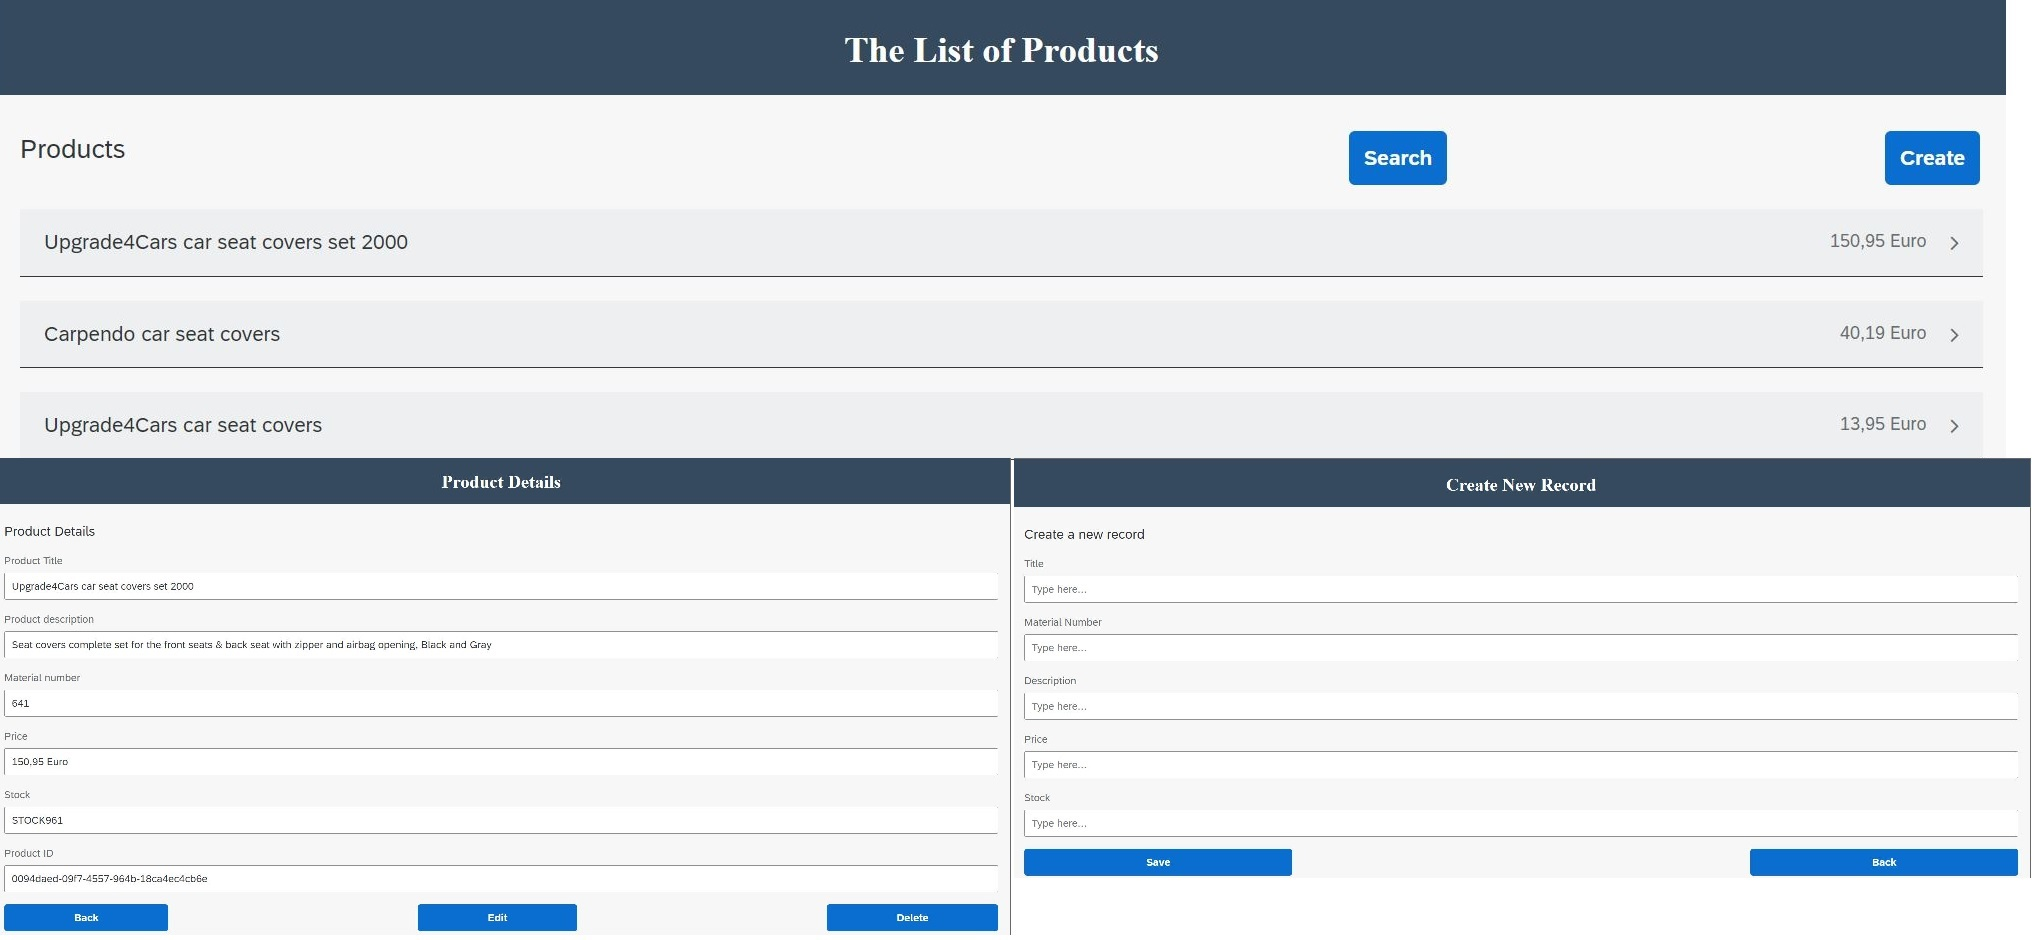
\includegraphics[width=1.0\textwidth]{Bilder/appgyver/3_18_appgyver_list.jpg}
 \caption{Listenseite, Detailseite und „Create new record“-Seite der AppGyver-Anwendung}
\end{figure}

\section{SAPUI5}
\subsection{Erstellung einer Anwendung mit dem UI5-Generator}
In Kapitel 2.5 wurden SAPUI5 und die Einrichtung der Entwicklungsumgebung für die Implementierung von SAPUI5-Anwendungen kurz vorgestellt. In diesem Abschnitt wird nun die Erstellung der SAPUI5-Applikation näher beschrieben.
Mit Hilfe des easy-ui5-Generators lässt sich ein grundlegendes SAPUI5-Anwendungsgerüst erstellen. Da die Entwicklung der Applikaton auf dem neuesten Stand der Technik erfolgen soll, wird TypeScript für das Coding verwendet. TypeScript ist eine Design-Time-Programmiersprache, die JavaScript um eine starke Typisierung erweitert. Das UI5-Typescript-Tooling nutzt den Babel-Compiler (JavaScript Compiler), um den TypeScript-Code in ausführbaren JavaScript-Code umzuwandeln \cite{pm:gswt}. Dabei läuft ein Prozess im Hintergrund, der die Quellen im src-Ordner überwacht und die transpilierten Dateien in den webapp-Ordner kopiert. 

Zur Erzeugung des Applikations-Gerüsts wird der Befehl \textit{yo easy-ui5 ts-app} in der Command-Prompt-Konsole ausgeführt. Dieser Befehl führt dazu, dass eine UI5-TypeScript-Anwendung basierend auf den folgenden Parametern erstellt wird:

\lstset{
  numbers=none, 
  basicstyle=\scriptsize,
  xleftmargin=.02\textwidth,
  backgroundcolor=\color{mygrey2},
}
\begin{lstlisting}[language=bash, caption=Eingabe der Paramtern des UI5-Generators]
? How do you want to name this application? products
? Which namespace do you want use? fanfan.products 
? Which framework do you want to use? SAPUI5 
? Which framework version do you want to use? 1.108.4 
? Who is the author of the application? Tan Fangfang 
? Would you like to create a new directory for the application? Yes
\end{lstlisting}

Nach Eingabe der Parameter müssen noch alle externen Bibliotheken via npm install installiert werden und dann kann die Entwicklung beginnen.

Der Generator erzeugt die grundlegende Projektstruktur eines SAPUI5-Projekts. Das MVC-Pattern findet sich auch im Dateisytem wieder. So liegen die Controller im Verzeichnis controller, die Views im gleichnamigen Verzeichnis und es ist ebenfalls ein model-Verzeichnis vorgehsehen. Dies wird jedoch im Projekt nicht verwendet, sondern es werden auf Standard Odata- und JSONModel zurückgegriffen \cite{sud:ao}. Daneben sind noch eine Reihe an Konfigurationsdateien vorhanden. Beispiele hierfür sind die „package.json“-Datei, sowie die „manifest.json“-Datei. 

\begin{lstlisting}[language=bash,  caption=Die grundlegende Projektstruktur eines SAPUI5-Projekts]
project-root
|- src
   |- controller
      |- App.controller.ts
      |- BaseController.ts
      |- Main.controller.ts
   |- i18n
   |- model
   |- view
      |- App.view.xml
      |- Main.view.xml
   |- Component.ts
   |- manifest.json
   |- index.html
|- [...]
|- package.json
|- README.md
|- ui5.yaml
\end{lstlisting}

Die Datei „manifest.json“ enthält die Grundkonfiguration der Anwendung, die für die Ausführung benötigt wird. Alle Modelle, Bibliotheken, die in der „manifest.json“-Datei konfiguriert sind, werden beim Starten der Anwendung automatisch geladen und instanziiert. Die „rootView“- und „routing“-Konfigurationen definieren die Hauptansicht der Anwendung, die nach Öffnen im Browser angezeigt wird, und die Navigation zwischen den Ansichten.

In der Datei „App.view.xml“ wird die Benutzeroberfläche der Hauptansicht der Anwendung definiert. SAPUI5 unterstützt mehrere View-Typen (XML, HTML, JavaScript, JSON). In diesem Projekt wird das XML-Format verwendet. Für jede Ansicht, die in der Anwendung verwendet wird, soll eine eigene View-Datei erstellt werden, und jede View wird von einem separaten Controller gesteuert. 

Das Öffnen der Webanwendung erfolgt durch Aufrufen der index.html-Seite   über einen Webserver im Browser.  Das UI5-Tooling bringt bereits einen lokalen Webserver mit, der via npm run start gestartet werden kann.  Abbildung 3.19 zeigt das Aussehen der erzeugten Anwendung, die bereits erste Inhalte hat, die angepasst und ersetzt werden müssen. Während die Anwendung läuft, kann der Code in VS-Code geändert und die Änderungen direkt danach direkt im Browser angesehen werden. 

\begin{figure}[htbp]
 \centering
 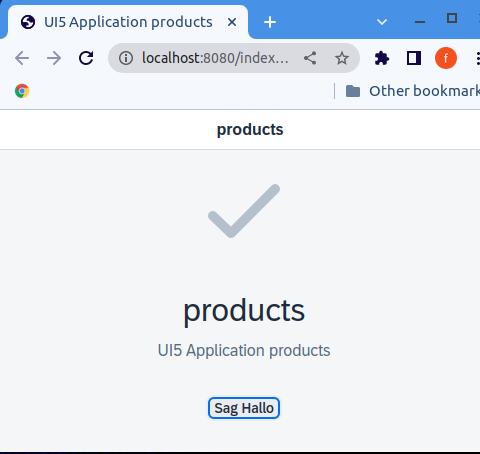
\includegraphics[width=0.4\textwidth]{Bilder/ui5 freestyle/3_19_ui5_demo.png}
 \caption{Aussehen der UI5 Demo-Anwendung}
\end{figure}

In den nächsten Abschnitten wird die Implementierung der UI5-Anwendung im Detail beschrieben. 

\subsection{OData-Service einbinden}

In Kapitel 3.2.2 wurde die Bereitstellung der OData-Services und der Destination in der SAP-BTP-Umgebung vorgestellt. Die SAPUI5-Anwendung muss diese Destination ebenfalls integrieren, um die OData-Services hinter der Destination konsumieren zu können. 

Leider lässt sich der OData-Server lokal nicht einfach im Browser einbinden, da dies zu einem Cross-Origin-Resource-Sharing (CORS)-Problem führt. Die Anwendung läuft unter der Domäne „localhost“ und moderne Browser erlauben es nicht, Daten via XMLHttpRequest von einer anderen Domäne zu laden (es sei denn, diese sendet entsprechende http-Header mit) \cite{sud:s25}. Um dieses Problem zu vermeiden, wird der Request über einen lokalen Reverse-Proxy (SAP Approuter) geleitet, der über das UI5-Tooling in das Projekt integriert werden muss. Dies ist zwar in wenigen Konfigurationschritten durchführbar, es zeigt aber bereits, dass auch gleich funktionierende Dinge (Zugriff auf die OData-Services via Destination) in SAPUI5 aufwendiger zu implementieren sind und die beiden LCNC-Toolings (Fiori Elements mit CAP und SAP AppGyver) derlei Dinge vom Entwickler fernhalten.

Der Zugriff auf die Daten in SAPUI5 erfolgt auf Basis eines OData-Models. Zwar ließen sich die Daten auch manuell als JSON abrufen, die Nutzung des OData-Models bietet jedoch den Vorteil, dass dies die http-Kommunikation komplett vom Entwickler fernhält. Zudem bietet das OData-Model weitere Features wie Databinding an, mit dem Daten sehr einfach an View-Controls gebunden und dargestellt werden können. 

Das OData-Model wird in der Component.ts-Datei erstellt und damit beim Starten der Anwendung initial in allen Controllern und Views bekannt gemacht.

\begin{lstlisting}[emph={oData},  caption=Auszüge aus der \texttt{Component.ts}]
const oData = new ODataModel({
  serviceUrl: "public/",
  synchronizationMode: "None",
  operationMode: "Server",
});
this.setModel(oData);
\end{lstlisting}

\subsection{Listenansicht zur Anzeige aller Produkte}
Die Listenansicht soll alle Produkte in einer Liste darstellen und es dem User ermöglichen, in die Einzelansicht eines Produkts zu springen. Da die Applikation nach dem Erstellen bereits über eine View verfügt, wird dies in der Main-View realisiert. Zentrales Element bildet die List-Control, welche Daten in einer Liste darstellen kann. Abbildung 3.20 zeigt die Benutzeroberfläche der Listenansicht der Produkte.

\begin{figure}[htbp]
 \centering
 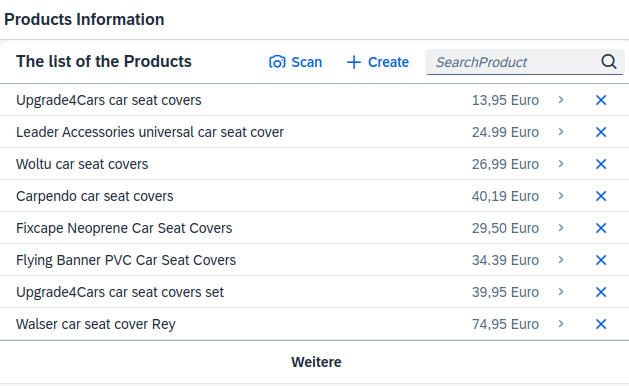
\includegraphics[width=0.8\textwidth]{Bilder/ui5 freestyle/3_20_Listeansicht.png}
 \caption{Benutzeroberfläche der Listenansicht der Produkte}
\end{figure}

SAPUI5-Controls sind UI-Elemente, die das Aussehen und Verhalten kapseln. In SAPUI5 stehen mehr als 100 Controls wie z.B. Buttons, Inputs, Texte, Tabellen, Messages, Dialoge, Listen usw. zur Verfügung. Eine Control kann andere Controls aggregieren und dient anschließend als Container. Die List-Control ist ein Container für entsprechende Listenelemente. Die Steuerung der View wird im entsprechenden Controller \textit{Main.controller.ts} implementiert. 

\begin{lstlisting}[language=XML,  caption=Auszüge aus der View \texttt{Main.view.xml}]
<List mode="Delete" delete="onDeletePress" items="{path:'/Products'}" id="productsList">
  <headerToolbar>
     <OverflowToolbar width="100%">
	<Title text="The list of the Products" />
	<ToolbarSpacer />
	<Button icon ="sap-icon://camera" text="Scan" press="onScanNavi"/>
         <Button icon="sap-icon://add" text="Create" ariaHasPopup="Dialog" press="pressAddInList" />
     <SearchField width="200px" placeholder="SearchProduct" search="mySearchProduct" />
     </OverflowToolbar>
  </headerToolbar>
<items>
  <StandardListItem title="{title}" type="Navigation" info="{price}" press="onItemPress"/>
</items>
</List>
\end{lstlisting}  

Das Coding zeigt den Ausschnitt der Listendefinition. Jede Control verfügt über bereitgestellte Eigenschaften (Properties) und Events, die im XML angegeben werden können. Mit der Eigenschaft \textit{mode="Delete"} wird beispielsweise automatisch ein Lösch-Button in der Liste hinzugefügt. Das Event \textit{delete=“onDeletePress“} verweist dahingehend dann auf die Callback-Funktion onDeletePress in der Klasse \textit{Main.controller.ts}, welche das Löschen dann programmatisch vornehmen muss:

\begin{lstlisting}[emph={event, UI5Event, listItem},  caption=Auszüge aus der Controller \texttt{Main.controller.ts}]
public onDeletePress(event: UI5Event) {
    const listItem = event.getParameter("listItem") as ColumnListItem;
    const context = listItem.getBindingContext() as Context;
    context.delete();
} 
\end{lstlisting}

In dieser Methode zeigt sich, dass in SAPUI5 durch die Models und das Databinding weder die Daten direkt aus den UI-Controls abrufen noch direkt mit dem OData-Service kommuniziert werden muss. Es wird an dieser Stelle lediglich der BindingContext (die Information zum Binding selber) benötigt und dieser aus dem Model gelöscht. Das sorgt dann automatisch dafür, dass das Model einen DELETE-Request zum OData-Service sendet und das Produkt aus der Datenbank entfernt wird.

Gleiches gilt auch für das initiale Setzen des Bindings. In obigem Coding zur Listenansicht ist zu sehen, dass in der Liste lediglich ein StandardListItem definiert wird. Dies dient dabei als Template für alle Produkte, die aus dem OData-Service ausgelesen werden. Über das Aggregation-Binding der Aggregation items (\textit{items="\{path:'/Products'\}"}) werden alle Produkte, sich in unter dem Pfad abrufen lasssen gebunden und für jedes Produkt wird ein \textit{StandardListItem} erzeugt, das den Titel und Preis anzeigt \cite{sud:s19}.

\begin{lstlisting}[language=XML,  caption=Auszüge aus der View \texttt{Main.view.xml}]
<StandardListItem title="{title}" type="Navigation" info="{price}" press="onItemPress"/>
\end{lstlisting}

Ein weiteres wichtiges Event ist das press-Event eines StandardListItems. Klickt ein User auf ein Produkt, so soll er auf die Detailseite weitergeleitet werden. Das zugehörige Coding zeigt, dass an dieser Stelle auf den Router zugegriffen wird. In SAPUI5 sorgt der Router dafür, dass URL-Pfade auf Views/Controller gemappt werden und ermöglicht es, dass das Framekwork im Hintergrund die notwendigen Controller/Views instanziiert.

\begin{lstlisting}[emph={event, UI5Event, listItem, detail, path}, caption=Auszüge aus der Controller \texttt{Main.controller.ts}]
public onItemPress(event: UI5Event){
    var item = event.getSource();
    var context = item.getBindingContext();
    var path = context.getPath().substr(1);
    this.navTo("detail", {path: path});
}
\end{lstlisting}

Auch hier wird auf das Binding zurückgegriffen, um Informationen zum Produkt auszulesen, die an die Detailseite übergeben werden.

\subsection{Einzelansicht für ein Produkt}
Damit die Navigation funktioniert, müssen für die Einzelansicht ein View \textit{Detail.view.xml} und ein Controller erstellt werden. In der View werden alle Merkmale, wie der Name, die Beschreibung, die Materialnummer, der Preis und der Bestand eines Produkts in den Input Controls angezeigt.
\begin{lstlisting}[language=XML, caption=Auszüge aus der View \texttt{Detail.view.xml}]
<Label text="Title" />    		
<Input value="{title}" width="1000px" />
<Label text="Description" /> 		
<Input value="{description}" width="1000px" />
<Label text="Material Number" />	
<Input value="{materialNumber}" width="1000px" />
<Label text="Price" />			
<Input value="{price}" width="1000px" />
<Label text="Stock" />		
<Input value="{stock}" width="1000px" />
\end{lstlisting}
Damit die Werte angezeigt werden können, wird in der View wieder ein ElementBinding verwendet, dass ein komplettes Produkt an die View bindet. Dann ist es ausreichend, lediglich die Attribute zu benennen und das OData-Model lädt die relevanten Daten automatisch. Abbildung 3.21 kann die finale Benutzeroberfläche der Einzelansicht für ein Produkt entnommen werden.
\begin{figure}[htbp]
 \centering
 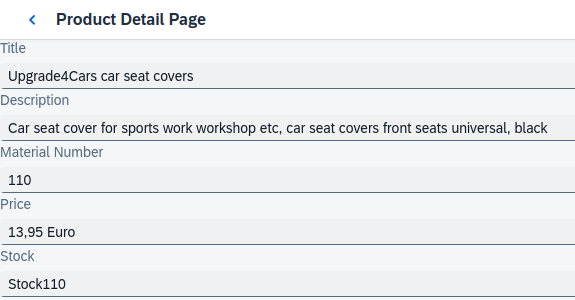
\includegraphics[width=0.8\textwidth]{Bilder/ui5 freestyle/3_21_Einzelansicht.png}
 \caption{Benutzeroberfläche der Einzelansicht}
\end{figure}

\subsection{Maske zum Pflegen eines einzelnen Produkts}

Für die Zusammenstellung der Maske zur Pflege eines Produkts werden Label-, Input- und Button-Controls und das Element \textit{Fragment} verwendet.  Fragmente sind leichtgewichtige UI-Komponenten, die wiederverwendbar sind, aber keinen Controller haben \cite{sud:s16}. Daher kann ein Fragment als ein Container für andere UI5-Controls betrachtet werden. Das UI-Design dieses Fragments ist in der Datei \textit{createProductDialog.fragment.xml} gespeichert.

\begin{lstlisting}[language=XML, caption=Auszüge aus der Fragment \texttt{createProductDialog.fragment.xml}]
<content>
  <VBox class="sapUiMediumMargin">
    <Label text="Title" />
    <Input value="{listInputModel>/recipient/title}" width="200px" />
    <Label text="Material Number" />
    <Input value="{listInputModel>/recipient/materialNumber}" width="200px" />
    <Label text="Description" />
    <Input value="{listInputModel>/recipient/description}" width="200px" />
    <Label text="Price" />
    <Input value="{listInputModel>/recipient/price}" width="200px" />
    <Label text="Stock" />
    <Input value="{listInputModel>/recipient/stock}" width="200px" />
  </Vbox>
</content>
<beginButton>
  <Button text="Cancel" ariaHasPopup="Dialog" press="closeDialog" />
</beginButton>
<endButton>
   <Button text="Add" ariaHasPopup="Dialog" press="pressAddInProductsList" />
</endButton>
\end{lstlisting}

In der Fragment-Implementierungsdatei werden mehrere Eingabefelder und zwei Buttons, \textit{Cancel} und \textit{Add} erstellt. Wird das press-Event des \textit{Add}-Buttons geworfen, so wird die Methode \textit{pressAddInProductsList} aufgerufen, um den Datensatz, der in das Eingabefeld eingegeben wurde, in den OData-Service zu übernehmen. Die Eingabewerte aller Eingabefelder werden zunächst via Binding an ein lokales JSON-Model übergeben. In der \textit{pressAddInProductsList}-Methode werden die Werte aus dem lokalen Model ausgelesen und ein neues OData-Binding erzeugt, dass die Daten automatisch an den OData-Endpunkt sendet.

\begin{lstlisting}[emph={var, ODataListBinding, materialNumber, items, recipient, listInputModel, title, id, description, price, stock}, caption=Auszüge aus der Controller \texttt{Main.controller.ts}]
public pressAddInProductsList() {
    var title = this.getView().getModel("listInputModel").getProperty("/recipient/title");
    var id = this.getView().getModel("listInputModel").getProperty("/recipient/id");
    var description = this.getView().getModel("listInputModel").getProperty("/recipient/description");
    var materialNumber = this.getView().getModel("listInputModel").getProperty("/recipient/materialNumber");
    var price = this.getView().getModel("listInputModel").getProperty("/recipient/price");
    var stock = this.getView().getModel("listInputModel").getProperty("/recipient/stock");

    const context = (<ODataListBinding>(
      this.getView().byId("productsList").getBinding("items")
      )).create({
        title: title,
        id: id,
        description: description,
        materialNumber: parseInt(materialNumber),
        price: price,
        stock: stock,
    });
    this.closeDialog();
}
\end{lstlisting}

Da das Formular zum Anlegen in einem Dialog geöffnet wird, muss dieser nach dem Absenden dann auch wieder geschlossen werden. Abbildung 3.22 zeigt das Dialogfenster zum Einfügen eines neuen Produkts.

\begin{figure}[htbp]
 \centering
 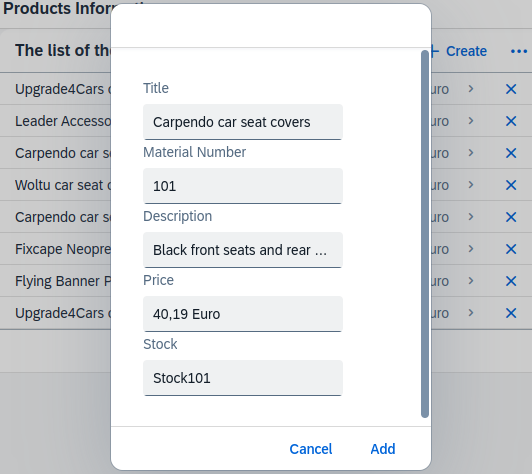
\includegraphics[width=0.6\textwidth]{Bilder/ui5 freestyle/3_22_Maske.png}
 \caption{Maske zum Pflegen eines einzelnen Produkts}
\end{figure}
















